\input{../common}

\begin{document}
  %<*content>
  \sheet{algebra, analysis}{denombrement}{Des outils du dénombrement}

  \summary{Aide-mémoire de dénombrement}

Pour dénombrer un ensemble, on peut utiliser: le comptage, un diagramme, un arbre de choix, un tableau à double entrée.\\
On peut aussi utiliser les trois outils fondamentaux:  p-listes,  arrangements,  combinaisons.\\ Chacun de ces outils  modélise  une situation fréquente  dans les problèmes de dénombrement: le tirage (ou choix) de $ p $ éléments dans un ensemble contenant  $ n $  éléments.

 Dans tous les cas devant un problème de dénombrement, on doit se poser les questions suivantes:
 
 \bigskip
 
 \begin{center}
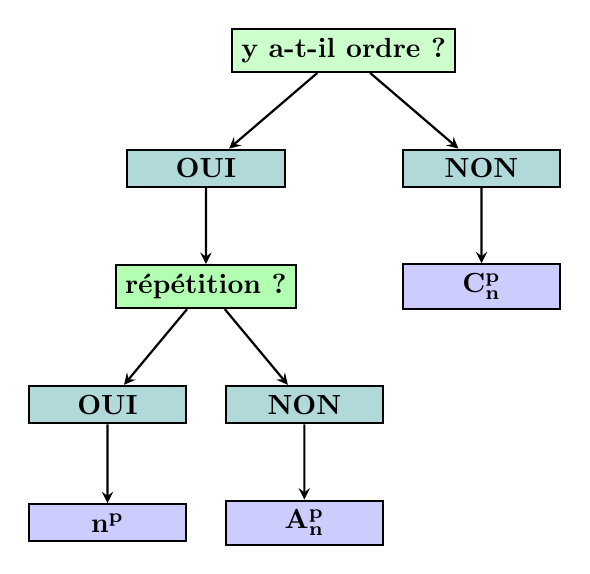
\begin{tikzpicture}[
  level 1/.style={sibling distance=35mm},
  level 2/.style={sibling distance=30mm},
  level 3/.style={sibling distance=25mm},
  edge from parent/.style={->, draw, thick, >=stealth, rounded corners=5pt},
  every node/.style={draw, thick, align=center, minimum width=2cm, fill=green!20}
]

\node {\textbf{y a-t-il ordre ?}}
  child {node[fill=teal!30]{\textbf{OUI}}
    child {node[fill=green!30]{\textbf{répétition ?}}
      child {node[fill=teal!30]{\textbf{OUI}}
        child {node[fill=blue!20]{$\mathbf{n^p}$}}
      }
      child {node[fill=teal!30]{\textbf{NON}}
        child {node[fill=blue!20]{$\mathbf{A_n^p}$}}
      }
    }
  }
  child {node[fill=teal!30]{\textbf{NON}}
    child {node[fill=blue!20]{$\mathbf{C_n^p}$}}
  };

\end{tikzpicture}

\end{center}
 
  
  $ n= $ nombre d'objets dans lesquels on tire, on choisit etc...\\
  $ p= $  le nombre d'objets à choisir ou quelques fois le nombre de tirages.\\
  
Les $A_{n}^{p} $ et  $C_{n}^{p} $ sont des entiers naturels qu'on peut calculer à l'aide de la calculatrice.\\

 Pour calculer $A_{n}^{p} $, on tape $ n\; n Pr\; p\; =$\\

 Pour calculer $C_{n}^{p} $, on tape  $ n\; n Cr\; p\; =$
 
 
 \textbf{Pour s'y retrouver dans les différents tirages :}
 Tirage de p éléments dans un ensemble à n éléments.
 \[
\begin{array}{|c|c|c|c|c|}
\hline
\textbf{Type} & \textbf{Ordre ?} & \textbf{Distincts ?} & \textbf{Outil} & \textbf{Nombre} \\
\hline
\text{Avec remise} & \text{Oui} & \text{Non} & \text{p-liste} & n^{p} \\
\hline
\text{Sans remise} & \text{Oui} & \text{Oui} & \text{Arrangement} & A_{n}^{p} \\
\hline
\text{Simultanés} & \text{Non} & \text{Oui} & \text{Combinaison} & C_{n}^{p} \\
\hline
\end{array}
\]


\begin{example}

 Une urne contient 3 boules bleues, 4 boules rouges et 2 boules vertes. Les boules sont supposées indiscernables au toucher.
 
 On tire simultanément trois boules de l'urne.
 
Combien y a- t-il de tirages  possibles:
\begin{enumerate}
\item contenant des boules de  la même couleur?
\item contenant des boules de couleurs  deux à deux distinctes?
\item  contenant deux boules rouges et une boule verte?
\end{enumerate}
\end{example}
\begin{proof}



 \textbf{Tirage simultané de trois boules parmi 9}.

 Les boules  sont tirées en même temps  donc il n'y a ni ordre ni répétition des 3 boules tirées.

Un tirage    correspond donc à une combinaison de 3 éléments dans un ensemble contenant 9 éléments. 

On utilise l'outil des combinaisons: donc il y a $ C_{9}^{3}= 84$ tirages possibles.
\begin{enumerate}
\item Nombre de tirages contenant des boules de même couleur.

 Les trois boules tirées sont bleues ou bien  sont rouges.
 
Le nombre de tirages est donc $ C_{3}^{3}+ C_{4}^{3} = 6+4=10$ . 
\item Nombre de tirages contenant des boules de couleurs deux à deux distinctes (ou nombre de tirages  tirage tricolore).

Un tirage ici est un élément du produit cartésien de trois ensembles: l'un constitué d'une boule bleue prise parmi 3  bleues et l'autre constitué d'une boule rouge prise parmi 4  rouges et le dernier d'une boule verte prise parmi 2  vertes.

Le nombre de tirages est donc $ C_{3}^{1}\times C_{4}^{1}\times C_{2}^{1}=3\times 4\times 2=24 $ .
\item  Nombre de tirages contenant deux rouges et une verte.\\
Un tirage ici est un élément du produit cartésien de deux ensembles: l'un constitué de 2 boules rouges prises parmi 4 et l'autre constitué d'une boule verte prise parmi 2.\\
Le nombre de tirages est donc  $ C_{4}^{2}\times C_{2}^{1}=6 \times 2 =12 $. 
\end{enumerate}
\end{proof}
\begin{example}

Une urne contient 3 boules bleues, 4 boules rouges et 2 boules vertes. Les boules sont supposées indiscernables au toucher.
 On tire successivement avec remise trois boules de l'urne.
Combien y a- t-il de tirages:
\begin{enumerate}
\item contenant des boules de même couleur?
\item contenant des boules de couleurs  deux à deux distinctes?
\item  contenant deux boules rouges et une boule verte?
\end{enumerate}
\end{example}

\begin{proof}


 \textbf{On tire successivement avec remise trois boules de l'urne.} 
 
On utilise l'outil des p-listes: donc il y a $ 9^{3}= 729$ tirages possibles.
\begin{enumerate}
\item Nombre de tirages contenant des boules de même couleur.\\
 Les trois boules tirées sont bleues ou bien  sont rouges ou bien  sont vertes.\\
Le nombre de tirages est donc  $ 3^{3}+ 4^{3}+ 2^{3} = 27+64+8=99$ .
\item Nombre de tirages contenant des boules de couleurs deux à deux distinctes.\\
Par exemple la première boule tirée est bleue prise parmi 3, suivie d'une deuxième boule   rouge prise parmi 4, suivie d'une troisième boule verte prise parmi 2: donc il y a $ 3^{1}\times 4^{1}\times 2^{1} $ tirages ayant la  configuration BRV. On obtient tous les tirages  tricolores possibles en multipliant ce résultat par le nombre d'anagrammes du mot BRV. \\
Le nombre de tirages est donc  $ 3^{1}\times 4^{1}\times 2^{1}\times 3!=3\times 4\times 2\times6=144 $. 
\item  Nombre de tirages contenant deux  boules rouges et une boule verte.\\
Par exemple on tire 2 boules rouges prises parmi 4 suivies d'une boule verte prise parmi 2: donc il y a $ 4^{2}\times 2^{1} $ tirages ayant la configuration RRV. Puis on obtient tous les tirages possibles comportant deux  boules rouges et une boule verte  en multipliant ce résultat  par le nombre d'anagrammes du mot RRV.\\
Le nombre de tirages est donc  $ 4^{2}\times 2^{1}\times \dfrac{3!}{2!}=16\times 2\times 3=96 $.
\end{enumerate}
\end{proof}



  %</content>
\end{document}
